\let\negmedspace\undefined
\let\negthickspace\undefined
\documentclass[journal]{IEEEtran}
\usepackage[a5paper, margin=10mm, onecolumn]{geometry}
%\usepackage{lmodern} % Ensure lmodern is loaded for pdflatex
\usepackage{tfrupee} % Include tfrupee package

\setlength{\headheight}{1cm} % Set the height of the header box
\setlength{\headsep}{0mm}     % Set the distance between the header box and the top of the text

\usepackage{gvv-book}
\usepackage{gvv}
\usepackage{cite}
\usepackage{amsmath,amssymb,amsfonts,amsthm}
\usepackage{algorithmic}
\usepackage{graphicx}
\usepackage{textcomp}
\usepackage{xcolor}
\usepackage{txfonts}
\usepackage{listings}
\usepackage{enumitem}
\usepackage{mathtools}
\usepackage{gensymb}
\usepackage{comment}
\usepackage[breaklinks=true]{hyperref}
\usepackage{tkz-euclide} 
\usepackage{listings}
% \usepackage{gvv}                                        
\def\inputGnumericTable{}                                 
\usepackage[latin1]{inputenc}                                
\usepackage{color}                                            
\usepackage{array}                                            
\usepackage{longtable}                                       
\usepackage{calc}                                             
\usepackage{multirow}                                         
\usepackage{hhline}                                           
\usepackage{ifthen}                                           
\usepackage{lscape}
\begin{document}

\bibliographystyle{IEEEtran}
\vspace{3cm}

\title{1-1.8-18}
\author{AI24BTECH11012 - Pushkar Gudla}
% \maketitle
% \newpage
% \bigskip
{\let\newpage\relax\maketitle}

\renewcommand{\thefigure}{\theenumi}
\renewcommand{\thetable}{\theenumi}
\setlength{\intextsep}{10pt} % Space between text and floats


\numberwithin{equation}{enumi}
\numberwithin{figure}{enumi}
\renewcommand{\thetable}{\theenumi}
\textbf{Question:} If the distance between the points $\myvec{4\\p}$ and $\myvec{1\\0}$ is $5$, then the value of $p$ is
\solution
\begin{table}[h!]    
  \centering
  \begin{tabular}[15pt]{ |c| c|}
    \hline
    \textbf{Variable} & \textbf{Description}\\ 
    \hline
    $a$ & Length of side $BC$ \\
    \hline 
    $b$ & Length of side $AC$ \\
	\hline
    $c$ & Length of side $AB$ \\
    \hline
	$k$ & $k=b-c$ \\
	\hline
    \end{tabular}

  \caption{Variables Used}
  \label{tab 1.8.18}
\end{table}
\begin{align}
	\vec{D}	&= \myvec{3\\p} \\
	\norm{\vec{D}}^2 &= \vec{D}\vec{D}^\top \\
	\norm{\vec{D}}^2 &= \myvec{3\\p}\myvec{3 & p} \\
	\norm{\vec{D}}^2 &= 3^2 + p^2 \\
	\implies \norm{\vec{D}}^2 &= 9 + p^2
\end{align}
It has been given that the distance between the two points is $5$, so \\
\begin{align}
	\norm{\vec{D}}^2 &= 25 \\
	\implies 25 &= 9 + p^2 \\
	\implies p &= \pm 4
\end{align}
\begin{figure}[h]
	\centering
	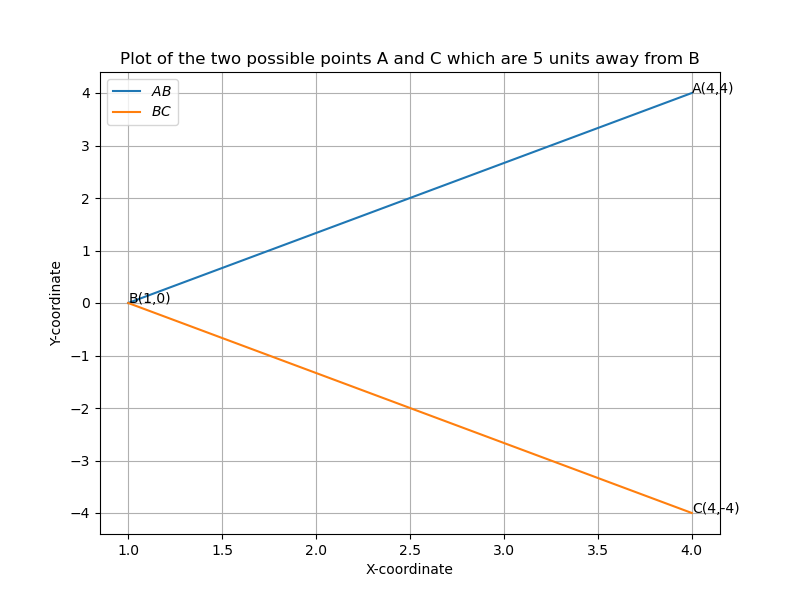
\includegraphics[scale=0.6]{figs/plot.png}
	\label{Fig}
\end{figure}
\end{document}
